% !TeX encoding = UTF-8
% !TeX program = pdflatex
% !TeX spellcheck = it_IT

\documentclass[binding=0.6cm,TFA]{sapthesis}

\usepackage{microtype}
\usepackage[italian]{babel}
\usepackage[utf8]{inputenc}
\usepackage[hidelinks]{hyperref}
\usepackage{setspace}
\usepackage[Algoritmo]{algorithm}
\usepackage{algorithmic}
\usepackage{graphicx}
\usepackage{listings}
\usepackage{dirtytalk}
\usepackage{xcolor}
\lstset { %
    language=C++,
    backgroundcolor=\color{black!5}, % set backgroundcolor
    basicstyle=\footnotesize,% basic font setting
}
\usepackage[chapter]{minted}

\renewcommand\listingscaption{Codice}

\onehalfspacing
\graphicspath{ {assets/} }

\hypersetup{pdftitle={Green IoT: Design e valutazione delle prestazioni di protocolli per sistemi IoT dotati di wake up radio},pdfauthor={Leonardo Emili}}

\title{Green IoT: Design e valutazione delle prestazioni di protocolli per sistemi IoT dotati di wake up radio}
\author{Leonardo Emili}
\IDnumber{1802989}
\course{Informatica L-31}
\courseorganizer{Facoltà di Ingegneria dell'informazione, informatica e statistica}
\AcademicYear{2019/2020}
\copyyear{2020}
\advisor{Prof. Chiara Petrioli}
\coadvisor{Dr. Georgia Koutsandria}
\authoremail{emili.1802989@studenti.uniroma1.it}

\begin{document}
\large

\frontmatter
\maketitle

% treat this as a special chapter
\chapter*{Ringraziamenti}

Vorrei iniziare ringraziando vivamente la \textbf{Prof. Chiara Petrioli} per il suo supporto e per l'ispirazione fornita senza i quali non avrei mai scoperto
le tematiche delle Wireless Sensor Network e affrontato un percorso simile. La sua ispirazione e le costanti sfide da risolvere durante questo lavoro di tirocinio
sono stati di fondamentale importanza sia per il progresso di questo progetto che per la mia crescita personale. Ci tengo inoltre a ringraziare di cuore la
\textbf{Dr. Georgia Koutsandria} per il continuo aiuto fornito e per l'enorme pazienza dimostrata nei miei confronti a fronte degli incessanti quesiti posti
durante questo tirocinio.\\

Senza dubbio la stesura di questa relazione non sarebbe mai stata possibile senza il continuo supporto dimostrato dai miei amici e dai parenti. Voglio
ringraziare in modo particolare la mia famiglia che mi è stata sempre vicina durante questo percorso di laurea e a cui devo tutto.

\let\cleardoublepage    % probably not a good decision
\clearpage
\let\cleardoublepage\clearpage  % restore changes

\tableofcontents

\mainmatter
\chapter{Introduzione}

Nell'ultimo decennio abbiamo assistito ad uno sviluppo portentoso del settore dell'Internet of Things che ha contribuito alla diffusione
di un enorme numero di dispositivi wireless. Il numero di questi dispositivi ha registrato crescite costanti negli anni e loro applicazioni sono ormai infinite.
Essi trovano impiego in ambito domestico dove realizzano l'automatizzazione dei compiti quotidiani, in quello sanitario in cui monitorano lo stato di salute
dei pazienti e in ambito sottomarino dove gli obbiettivi spaziano da quello di realizzare campionamenti di dati sino a creare vaste reti di comunicazione sottomarine.
L'immissione di questo enorme contingente di dati nella rete ha reso possibili nuove interpretazioni del mondo che ci circonda e lo sviluppo di soluzioni che puntano
a migliorare la qualità della vita delle persone, anche in quei settori noti esser di difficile comprensione. Ad esempio, l'impiego di sensori IoT in ambito di
monitoraggio del crosta terrestre ha reso disponibili informazioni fino a prima sconosciute sulla presenza di terremoti e tsunami, migliorando radicalmente
la nostra percezione degli eventi sismici nel mondo.\\

Con lo sviluppo massivo dell'IoT nuove sfide sono emerse a minare la solidità degli approcci usati. Attualmente le soluzioni impiegate nello sviluppo
dei dispositivi wireless puntano a realizzare comunicazioni con basse latenze e che siano altamente efficienti in termini energetici. In ambito di ricerca,
lo stato corrente dell'arte punta a realizzare tecnologie hardware e software che implementino questo binomio. Un particolare
settore dell'IoT si occupa di realizzare vaste reti di nodi sensori interconnessi, note come \emph{Wireless Sensor Network},
che realizzano una comunicazione wireless con consumi minimi al fine di prolungare i tempi di servizio dell'intera rete. In questo caso,
le principali problematiche sono chiaramente settoriali e sono identificate dallo specifico campo di applicazione: come la richiesta di tecnologie
altamente performanti per i monitoraggi clinici oppure di altre che garantiscano elevate lifetime nel caso di sensori ambientali. Tuttavia esistono
problematiche comuni a queste tipologie di reti, ad esempio spesso si richiede che l'intera rete sia connessa e che tutti i nodi siano,
anche parzialmente, a conoscenza della topologia della rete. Si richiede quindi l'impiego di protocolli che ne prevedano il
costante aggiornamento e favoriscano una comunicazione efficiente. Inoltre, in queste reti la principale fonte di consumo energetico risiede
nella comunicazione tra nodi ma anche nel cosiddetto \emph{idle listening}, ovvero il tempo in cui i nodi sono attivi con il trasmettitore pronto a
ricevere senza che sia in corso alcuna comunicazione: è quindi di vitale importanza prevedere lo scaricamento delle batterie che li alimentano
e studiare soluzioni che ne favoriscano durate sufficientemente elevate per garantire l'operatività della rete. Infatti, la morte prematura di un nodo
può spesso avere conseguenze più grandi della semplice disconnessione dello stesso poiché frequentemente si tratta di reti \emph{multi-hop} che
realizzano la comunicazione passando attraverso nodi intermedi ed in alcuni casi si può verificare perfino la disconnessione dell'intera rete.\\

In questa tesi ci siamo concentrati su un paradigma emergente per ottimizzare il trade-off energia-latenza nelle reti di nodi sensori: i dispositivi IoT
dotati di wake up radio, in grado di essere selettivamente svegliati solo quando il nodo deve compiere task (quali la ricezione di un messaggio). I nuovi
dispositivi IoT dotati di wake up radio creano le premesse per ottimizzazioni delle prestazioni delle reti di sensori finora non possibili. Nell'ambito
della tesi è stato implementato nel simulatore Green Castalia uno dei primi protocolli proposti per tali sistemi, ne sono state studiate le prestazioni.
In base allo studio simulativo sono state proposte nuove varianti che ne ottimizzano le prestazioni.\\

Nel seguito sarà brevemente descritta la struttura del documento e saranno enumerati per ciascun capitolo i contenuti in esso presenti.\\

Nel \textbf{Capitolo 2} viene introdotto lo scenario di riferimento e sono presentate soluzioni allo stato dell'arte in ambito di protocolli di rete. In questo
capitolo discutiamo delle principali considerazioni che nel tempo sono state adottate e che ad oggi definiscono il panorama delle Wireless Sensor Network.\\

Nel \textbf{Capitolo 3} viene analizzato uno specifico protocollo di rete per sistemi IoT: il protocollo GREEN-WUP, presentato in \cite{novel-wake-up-receiver-paper}.
In questo lavoro ci concentreremo sullo studio dei principi che regolano il design dei protocolli di rete e sulla loro applicazione in riferimento al
protocollo in questione. In questo capitolo viene analizzato in dettaglio il comportamento del protocollo e le sue caratteristiche. Vengono inoltre presentati i
suoi principali vantaggi e le soluzioni da esso proposte proposte per affrontare le problematiche comuni ai protocolli di comunicazione.\\

Nel \textbf{Capitolo 4} viene presentata una nuova variante del protocollo originale che punta a risolvere le problematiche osservate nel capitolo precedente.
Vengono descritte in dettaglio le modifiche apportate sia a livello teorico che a livello di implementazione all'interno di Castalia che è
il simulatore utilizzato e a cui faremo diffusamente riferimento all'interno di questa relazione. In particolare, tutto il codice
a cui si fa riferimento in questo documento è stato testato mediante una versione particolare del framework \emph{GreenCastalia} \cite{greencastalia-paper}
che supporta \emph{wake up radio} e \emph{energy harvesting}.\\

Nel \textbf{Capitolo 5} vengono misurate le prestazioni delle implementazioni del protocollo GREEN-WUP e della variante proposta,
confrontati i risultati ottenuti in relazione ad alcune metriche fondamentali e descritto l'ambiente di simulazione.\\

Nel \textbf{Capitolo 6} vengono presentati i parametri dei protocolli di rete che in misura principale contribuiscono alle loro prestazioni e ne favoriscono
il risparmio energetico. Parte fondante di questo tirocinio consiste nella sperimentazione tramite simulatori del comportamento che questi protocolli
assumono in ambito reale. In questi termini questo capitolo punta ad ottimizzare i parametri utilizzati nell'implementazione del protocollo GREEN-WUP e
che in generale rispecchiano i comportamenti comuni ai protocolli di rete utilizzati al giorno d'oggi.\\

Nel \textbf{Capitolo 7} vengono presentate le conclusioni del lavoro e discussi i possibili sviluppi futuri.

\let\cleardoublepage    % probably not a good decision
\clearpage
\let\cleardoublepage\clearpage  % restore changes

\chapter{Scenario di riferimento}

Sino a qualche anno fa, la principale tendenza nello sviluppo di soluzioni ai problemi menzionati nel \textbf{Capitolo 1} consisteva nell'introduzione di cicli di attività
dei nodi. Il cosiddetto \emph{duty cycling}, definito come la frazione di tempo in cui un nodo è attivo, aveva come obiettivo quello di minimizzare i momenti
in cui i nodi sensori sono accesi senza alcuna trasmissione o ricezione di pacchetti o processing dei dati in corso. Seppur questo approccio permetta di prolungare la durata della vita della rete,
incrementa in maniera considerevole i ritardi nelle comunicazioni, dal momento che queste possono avvenire solamente all'interno delle finestre di attività
delle coppie dei nodi coinvolti.\\

In questo panorama viene introdotta la tecnologia rivoluzionaria delle \emph{wake up radio}, il cui obbiettivo consiste nell'eliminazione dei consumi energetici
superflui relativi alle attese che precedono la ricezione dei pacchetti. L'idea prevede che i nodi della rete siano prevalentemente dormienti durante il loro
periodo di attività e che attivino la radio principale solamente per ricevere oppure per inviare un pacchetto dati. Di fatto questo meccanismo implementa uno
schema di comunicazione \emph{on demand}: un nodo può inviare un pacchetto dati ad un nodo dormiente semplicemente posticipandone l'invio a quello di una
sequenza di wake-up che, svegliando il ricevente, lo abilita alla ricezione. Infine, allo scadere del tempo necessario per permettere al nodo di ricevere il
pacchetto, la radio principale viene nuovamente posta in stato di SLEEP per risparmiare energia.\\

L'utilizzo delle wake up radio prevede l'introduzione di una radio secondaria a bassissimo consumo energetico il cui compito consiste solamente nel processamento dei messaggi di wake up ricevuti
da parte dei nodi della rete. Quest'ultima in particolare rimane costantemente accesa per poter in ogni momento ricevere delle sequenze di wake up, permettendo
quindi di lasciare disattiva la radio principale per tutto il tempo in cui questa non è necessaria. Si noti come spesso dal punto di vista di design
dell'hardware si preferisce separare la logica di wake up da quella della radio principale. In questi casi viene progettata una nuova antenna di dimensioni
ridotte e consumi energetici nettamente inferiori rispetto a quelli della radio principale che si occuperà di ricevere i messaggi di wake up.\\

Dal punto vista energetico il meccanismo delle wake up radio è altamente efficiente e non richiede alcuna forma di sincronizzazione che generalmente
risulta essere  non desiderata in quanto implicitamente introduce overhead dovuto alla gestione di timer aggiuntivi.\\

Successivamente la tecnologia delle wake up radio è stata ulteriormente sviluppata attraverso l'impiego del cosiddetto \emph{semantic addressing}.
L'idea in questo caso consiste nell'associare la ricezione di una sequenza di wake up ad un sottoinsieme di nodi della rete, evitando quindi che questa sia
recepita da tutti i nodi presenti all'interno del range di comunicazione. Il principio fondante è quello di scegliere uno o più opportuni indirizzi di
wake up e di assegnarli ad un certo sottoinsieme di nodi della rete. A meno di errori di interpretazione della sequenza di wake up, al momento della
ricezione tutti e soli i nodi desiderati saranno svegliati. In questo scenario i consumi energetici risultano essere ulteriormente ridotti poiché viene
virtualmente azzerato il numero dei nodi che vengono riattivati in seguito alla ricezione di messaggi di wake up, limitando l'attivazione ai soli nodi che
per capacità o risorse attuali (es energetiche) sono i più idonei ad  eseguire dei task (di processing e/o comunicazione).\\

Più recentemente la tendenza è quella di equipaggiare i nodi delle Wireless Sensor Network con moduli per l'\emph{energy harvesting} come ulteriore
supporto energetico alla loro durata di attività. In particolare, i nodi sono in grado di utilizzare l'energia fornita dalle batterie di cui sono
forniti e di derivarne nuova mediante turbine eoliche, pannelli solari e generatori termoelettrici di cui sono equipaggiati.\\

\newpage
La presenza di moduli per l'energy harvesting abilita le Wireless Sensor Network a disporre di lifetime che fino a prima non erano state mai sperimentate.
Infatti, sebbene l'energia derivata da sorgenti esterne sia di ordini di grandezza inferiore rispetto a quella fornita dalle batterie di cui i nodi sono
equipaggiati, i moduli di energy harvesting sono di vitale importanza per i nodi della rete. Essi permettono persino di risolvere problemi di disconnessione
della rete in quanto possono recuperare quei nodi diventati inattivi a seguito dello scaricamento delle batterie di cui sono forniti. In
\cite{wsn-energy-harvesting-paper} viene descritto l'enorme contributo che l'impiego di moduli di energy harvesting può fornire alle lifetime delle
Wireless Sensor Network, arrivando anche a permettere loro durate di diversi anni e persino decenni.\\

In ambito di ricerca sono presenti molti articoli scientifici in cui viene indagata la transizione dall'utilizzo del duty cycling alle wake up radio. Ad esempio
in \cite{beyond-duty-cycling-paper} viene presentato il protocollo ALBA-WUR, come estensione del protocollo ALBA-R, che utilizza la tecnologia delle wake up radio
e che ha come obbiettivo quello di ridurre l'energia spesa dalla rete e fornire lifetime superiori rispetto a quelle precedentemente sperimentate. In
\cite{ctp-wur-paper} viene proposto il protocollo CTP-WUR, come estensione al classico protocollo CTP, che utilizza le wake up radio piuttosto che il
duty cycling per prolungare la lifetime delle Wireless Sensor Network.\\

Ad oggi sono molti i protocolli che adottano la tecnica del semantic addressing come soluzione per ridurre i costi energetici della rete. Tra questi
vale la pena nominare alcune pubblicazioni scientifiche, tra cui: \cite{novel-wake-up-receiver-paper}, \cite{beyond-duty-cycling-paper}, e \cite{ctp-wur-paper}.
In ciascuno di questi paper vengono evidenziati i benefici energetici derivanti dall'utilizzo della tecnica del semantic addressing. È stato inoltre
dimostrato che l'impiego di nodi dotati di energy harvesting \cite{energy-harvesting-paper} e che sono abilitati alle wake up radio
\cite{wake-up-radios-paper} ha portato notevoli incrementi nelle prestazioni sperimentate nelle Wireless Sensor Network.\\

Questo lavoro si concentra sullo studio di protocolli delle cosiddette \emph{green wireless sensor network}, ovverosia di quei protocolli che si basano
sulle tecnologie sopra esposte e che implementano la comunicazione tra nodi minimizzandone gli sprechi energetici. Nella letteratura scientifica
sono presenti molti protocolli di questo tipo (es. CTP-WUR \cite{ctp-wur-paper}, GREENROUTES \cite{wake-up-radios-paper}, WHARP \cite{wharp-paper}) che
presentano euristiche distribuite o tecniche di ottimizzazione basate su \emph{reinforcement learning} per ottimizzare lo scambio dati in reti IoT dotate di wake
up radio e energy harvesting.

\chapter{Il protocollo GREEN-WUP}

\section{Interest dissemination}

In questa sezione viene presentato il meccanismo di interest dissemination che viene utilizzato per determinare gli hop count dei nodi della rete,
ovverosia la distanza in hop dei nodi rispetto al sink node. Ciò avviene mediante l'impiego di un protocollo di flooding chiamato FLOOD-WUP
\cite{novel-wake-up-receiver-paper} che permette di distribuire pacchetti a tutti i nodi della rete senza incorrere in \emph{broadcast storm}.\\

L'obbiettivo della fase di interest dissemination è di assegnare a ciascun nodo della rete un valore di hop count. Nel caso di FLOOD-WUP ciò
avviene secondo un algoritmo iterativo: questo avrà valore 0 nel solo caso del sink node, altrimenti assume un valore $h$ se $h-1$ è il valore
di hop count del nodo precedente.

%image source: https://www.researchgate.net/figure/Topology-of-wireless-sensor-network-and-hop-count-of-sensors_fig7_285956270
\begin{figure}[h]
    \begin{center}
        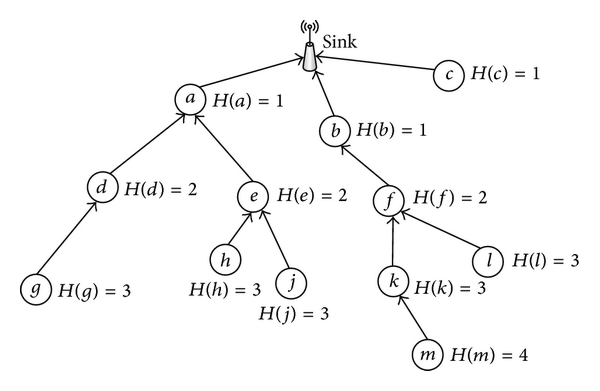
\includegraphics[scale=1.8]{hop-count-algorithm.png}
        \caption{Topologia della rete a seguito dell'assegnazione degli hop count. Sorgente: \cite{hop-count-figure}}
    \end{center}
\end{figure}

L'inizio della fase di interest dissemination viene sancito nel momento in cui il sink node invia un primo pacchetto attraverso cui richiede
ai nodi della rete di iniziare a determinare il proprio hop count. Suddetto pacchetto prende il nome di \emph{command packet} e contiene
al suo interno un campo contenente il valore di hop count del nodo che lo ha inviato. L'hop count vale inizialmente zero 
e viene incrementato di uno ad ogni nuova ricezione da parte degli altri nodi. In questo modo è possibile assegnare gli hop count ai nodi
della rete semplicemente seguendone la definizione ricorsiva.\\

Si noti come in FLOOD-WUP il traffico generato non provochi broadcast storm e ciò è possibile grazie all'impiego dei messaggi
di wake up. Infatti, ciascun nodo fa riferimento ad una pool di indirizzi di wake up condivisa $w_1, w_2, \cdots, w_n$ e ha inizialmente
settato come indirizzo di wake up $w_1$. Quando il primo pacchetto di interest viene inviato dal sink node si utilizza $w_1$ come sequenza
di wake up che lo precede. Al momento della ricezione del pacchetto, i nodi cambiano il loro indirizzo di wake up in $w_2$ e lo redistribuiscono
precedendolo con la stessa sequenza di wake up con la quale è stato spedito. Il successivo pacchetto viene spedito dal sink
node utilizzando $w_2$ come sequenza di wake up e questo evita di ricevere pacchetti duplicati in quanto i nodi che hanno già ricevuto un
pacchetto non saranno successivamente svegliati da quella stessa sequenza di wake up.\\

\begin{listing}
    \caption{Codice di aggiornamento della sequenza di wake up utilizzata dal sink node per distribuire il command packet.}
    \begin{minted}[mathescape,
                   linenos,
                   numbersep=10pt,
                   gobble=0,
                   fontsize=\small,
                   frame=lines,
                   framesep=2mm]{cpp}
// New packet received from the upper layer (either a DATA or INTEREST pkt)
GreenWupPacket *macFrame;
if (isSink) {
    // This is a dissemination packet - Update associated wur
    macFrame = new GreenWupInterest("GreenWupInterest", MAC_LAYER_PACKET);
    macFrame->setWurAddress(wurDisseminationAddresses[fromNetAddressIndex]);
    int n = wurDisseminationAddresses.size();
    fromNetAddressIndex = (fromNetAddressIndex + 1) % n;
    macFrame->setType(PKT_GREEN_WUP_INTEREST);
    // Initialize the hop count to 0
    macFrame->setHopCount(level);
} else {
    macFrame= new GreenWupData("GreenWupData", MAC_LAYER_PACKET);
    macFrame->setType(PKT_GREEN_WUP_DATA);
}

// Add MAC header and provide the required fields
encapsulatePacket(macFrame, pkt);
macFrame->setDestination(destination);
macFrame->setNetAddress(self);
macFrame->setNetSN(netSN++);
macFrame->setSource(SELF_MAC_ADDRESS);

    \end{minted}
\end{listing}

\begin{listing}
    \caption{Codice di aggiornamento della sequenza di wake up usata dai nodi.}
    \begin{minted}[mathescape,
                   linenos,
                   numbersep=10pt,
                   gobble=0,
                   fontsize=\small,
                   frame=lines,
                   framesep=2mm]{cpp}
// Interest packet received from the network
GreenWupInterest *macPkt = dynamic_cast <GreenWupInterest*>(pkt);

// Update current hop count
updateLevel (macPkt->getHopCount());

// Ignore duplicated packtes
if (isNotDuplicatePacket(pkt) == false) {
    // Drop duplicate packets (i.e. received while doing CSMA/CA)
    return;
}

// Update next hop count
GreenWupInterest *newPkt = dynamic_cast <GreenWupInterest*>(pkt->dup());
newPkt->setHopCount(level);

// Update current wur address (replace i-th address with address (i+1) mod n)
wurModule->removeWakeupAddress(wurDisseminationAddresses[addressIndex]);
addressIndex = (addressIndex + 1) % (wurDisseminationAddresses.size());
wurModule->addWakeupAddress(wurDisseminationAddresses[addressIndex]);

    \end{minted}
\end{listing}

\let\cleardoublepage    % probably not a good decision

La porzione di codice in \textbf{Codice 3.1} mostra il comportamento del sink node quando questo genera un command packet. L'idea in questo caso è
di generare dei command packet che saranno trasferiti sino al livello \emph{data link} per essere instradati nella rete. Dunque il sink node procede
fornendo i campi richiesti alla creazione del pacchetto di interest ed in particolare setta la tipologia del pacchetto da inviare in quanto sarà poi
utile in fase di ricezione dei pacchetti per evitare confusioni e stabilire quale operazione applicare al pacchetto ricevuto.
Infine il sink node inizializza il valore del campo \emph{hopCount}, aggiorna il prossimo indirizzo wake up da utilizzare ed invia il pacchetto in broadcast.\\

\newpage
Si noti come generalmente vengono generati un numero $m \geq 1 $ di command packet per assicurarsi che tutti i nodi della rete siano raggiunti. Ciascun pacchetto
di interest viene spedito ad una distanza di tempo $\delta$ dal pacchetto precedente. Infatti, il valore assegnato a $\delta$ deve essere sufficientemente
grande per permettere che la precedente fase di interest sia terminata nel momento in cui inizia una nuova. Nell'implementazione presentata in questo lavoro
si è scelto di utilizzare $m=3$ e $\delta=60s$.\\

Dualmente in \textbf{Codice 3.2} il pacchetto di interest viene ricevuto controllando il valore del campo \emph{type} del pacchetto in questione. Viene
successivamente chiamata la funzione \emph{updateLevel} che aggiorna il valore di hop count del nodo considerando il suo valore di hop count
e quello presente all'interno del pacchetto e prendendone il minimo tra i due. Infine viene aggiornato il valore di hop count contenuto
nel pacchetto e sostituita la sequenza di wake up con cui il nodo è stato svegliato con la sequenza successiva. Si noti come 
nell'implementazione mostrata sia presente un controllo per evitare di ritrasmettere pacchetti duplicati mentre nella descrizione originale
questo comportamento non viene descritto. Quanto accade è assolutamente possibile e non è da imputare allo specifico protocollo: può capitare infatti
che un nodo sia già attivo (RX) poiché stava precedentemente facendo carrier sensing del canale di comunicazione ed in queste condizioni
potrebbe ricevere un pacchetto senza ricevere prima alcuna sequenza di wake up, risultando di fatto nella ricezione di pacchetti duplicati.

\let\cleardoublepage\clearpage  % restore changes

\section{Descrizione del protocollo}

Il protocollo GREEN-WUP si inserisce nel contesto dei protocolli delle \emph{green wireless sensor network} e pone tra i suoi principali obiettivi
la massima efficienza energetica della rete. Esso impiega le tecnologie di wake up radio, energy harvesting e semantic addressing. Inoltre, è
di tipo \emph{converge casting} ed è basato sull'assegnazione di hop count a ciascun nodo per poter distribuire i pacchetti dati
all'interno della rete.\\

L'approccio tradizionale dei protocolli di rete prevede due fasi principali: in primo luogo avviene la fase di \emph{interest dissemination} dove si
definisce la topologia della rete da rispettare affinché i nodi realizzino un corretto flusso di scambio dati; successivamente si assume che gli
indirizzi di wake up siano stati assegnati e si procede con lo scambio di dati che è governato da sequenze di wake up che vengono utilizzate per
risvegliare i nodi della rete. Nel caso specifico di GREEN-WUP la fase di interest dissemination non viene eseguita per motivi di efficienza
e gli hop count vengono determinati indirettamente prima ancora dell'inizio della simulazione. Per ragioni completezza in questo lavoro viene
mostrata sia la versione originale di GREEN-WUP che non comprende la fase di interest dissemination che una versione che la utilizza per
il calcolo degli hop count dei nodi della rete.\\

In GREEN-WUP ciascun nodo è fornito di una coppia di indirizzi di wake up. Si tratta infatti di un primo indirizzo che identifica univocamente
il nodo nella rete e rimane invariato nel tempo, e di un altro che è mutabile nel tempo ed è definito a partire dallo stato corrente del nodo.
Quest'ultimo indirizzo di wake up è definito da una sequenza $w=w_{h}w_{e}$ della lunghezza di 8 bit, dove $w_{h}$ rappresenta il valore di hop
count $h$ del nodo in questione, $w_{e}$ invece rappresenta la sua attuale classe energetica. In particolare, ciascun nodo considera
l'energia disponibile come quella rimanente nelle batterie assieme a quella derivata da sorgenti esterne. In definitiva, la codifica del suffisso
$w_{e}$ viene calcolata a partire dalla discretizzazione in $k$ classi della disponibilità energetica di un nodo, dove $k$ rappresenta il
numero delle classi disponibili. Si noti come quest'ultimo indirizzo venga periodicamente aggiornato per riflettere la disponibilità
energetica del nodo nel tempo. Questa idea realizza il principio del semantic addressing poiché in questo scenario è possibile far riferimento
ad un sottoinsieme di nodi della rete a partire dai loro valori di hop count e da quello della classe energetica. \\

Nel momento in cui un nodo deve inviare un pacchetto dati può farlo seguendo degli step fondamentali di seguito descritti.
La prima fase consiste nell'instaurare una comunicazione con i nodi eleggibili, idonei alla ritrasmissione del pacchetto: il suddetto nodo sensore
entra in uno stato di ricerca di un nodo che si farà carico della sua richiesta di ritrasmissione. La ricerca si considera conclusa
nel momento in cui viene selezionato un nodo tra quelli disponibili come nodo intermedio tra il nodo che invia i dati (sender) e il sink
node, cui la richiesta di ricezione dati è destinata. Infine si procede alla trasmissione del pacchetto, a seguito della quale
verrà inviata una conferma a certificare l'avvenuta ricezione dello stesso, ripetendo quindi questa procedura sino a raggiungere
il sink node.\\

Nel seguito sarà descritto il comportamento del protocollo da un punto di vista algoritmico ed in seguito saranno esposte alcune osservazioni su di esso.
Per facilitarne la lettura, il duplice ruolo che ciascun nodo assume viene scomposto in due parti: rispettivamente in \textbf{Algoritmo 1}
viene descritto il comportamento che ciascun nodo assume nel momento in cui deve inviare dei dati (sender), mentre in \textbf{Algoritmo 2}
viene descritto il comportamento che questo assume quando agisce da nodo intermedio (receiver).

\begin{algorithm}
    \caption{Sender in GREEN-WUP}
    \begin{algorithmic}
        \REQUIRE $level > 0$

        \WHILE{queue is not empty}
            \STATE $dataPkt \leftarrow$ queue.head()

            \IF{level = 1}
                \STATE send $dataPkt$ to the sink node and wait for some time $\delta_{ACK}$ to receive the relative ACK packet

            \ELSE
                \STATE $k \leftarrow$ maxEnergyClass
                \STATE $acked \leftarrow$ false
                \WHILE{$k>0$ $and$ not $acked$}
                    \STATE $address_{RTS} \leftarrow$ createWurAddress(level - 1, k)
                    \STATE send $address_{RTS}$ and wait for nearby nodes to wake up
                    \STATE $rtsPkt \leftarrow$ createRTS(self)
                    \STATE send $rtsPkt$ in broadcast and wait for some time $\delta_{CTS}$
                    
                    \IF{CTS packet is received within $\delta_{CTS}$}
                        \STATE send a wake up signal using the address contained inside the first CTS packet received and wait for the receiver to wake up
                        \STATE send $dataPkt$ and wait for some time $\delta_{ACK}$

                        \IF{ACK packet is received within $\delta_{ACK}$}
                            \STATE $acked \leftarrow$ true
                        \ENDIF
                    \ENDIF
                    \STATE $k \leftarrow k-1$
                \ENDWHILE
            \ENDIF
        
        \ENDWHILE
    \end{algorithmic}
\end{algorithm}

Si noti come in \textbf{Algoritmo 1} si abbia come precondizione fondamentale che il valore di hop count (\emph{level}) sia maggiore strettamente
di zero in quanto il design del protocollo prevede che il sink node agisca da mero destinatario nelle comunicazioni della rete. Nel caso in cui
il nodo è a diretto contatto con il sink node ($level=1$) la trasmissione del pacchetto dati avviene senza alcuna forma di
selezione del nodo intermedio, in quanto superflua. D'altra parte se il nodo non può trasmettere direttamente il pacchetto al sink node ($level>1$)
si procede contattando i nodi vicini al nodo in questione. I nodi candidati vengono considerati in base alla loro classe energetica corrente:
a partire dai nodi con classe energetica massima si procede poi considerando i nodi con classi energetica inferiore. Infine si noti come i nodi in fase
di trasmissione di pacchetti RTS/CTS includano gli indirizzi univoci (i rispettivi ID) mediante i quali potranno essere ricontattati attraverso una
comunicazione in \emph{unicast}.

\begin{algorithm}
    \caption{Receiver in GREEN-WUP}
    \begin{algorithmic}
        \REQUIRE the node detects a wake up signal $address_{RTS}$

            \STATE activate the main radio and wait for some time $\delta_{RTS}$

            \IF{RTS packet is received within $\delta_{RTS}$}
                \STATE $\delta_{JITTER} \leftarrow$ random value in $[0,maxJitter)$
                \STATE wait for $\delta_{JITTER}$ and then send a wake up signal using the address contained inside the RTS packet
                \STATE $ctsPkt \leftarrow$ createCTS(self)
                \STATE send $ctsPkt$ and wait for some time $\delta_{DATA}$

                \IF{DATA packet is received within $\delta_{DATA}$}
                    \STATE send an acknowledgement packet to the sender
                \ENDIF
            \ENDIF

            \STATE process buffered packets if there are any, otherwise go back to sleep
        
    \end{algorithmic}
\end{algorithm}

Osservando invece \textbf{Algoritmo 2} si può notare che all'inizio il nodo ricevente intercetti una sequenza di wake up a lui destinata. In risposta
al segnale di wake up ricevuto, il nodo ricevente attiva la radio principale (RX) ed attende di ricevere un pacchetto RTS. Si noti come il
protocollo preveda la presenza di un jitter randomico per evitare che avvengano collisioni durante la trasmissione dei pacchetti CTS da parte
dei nodi candidati. Analogamente a quanto sopra descritto i nodi riceventi includono un indirizzo univoco a cui essere eventualmente ricontattati.\\

Si noti come le descrizioni teoriche del protocollo sopra esposte non comprendano alcuni dettagli inerenti al meccanismo di trasmissione
dei pacchetti. In particolare, tra questi troviamo la tecnica di \emph{Carrier Sensing} (CSMA/CA) utilizzata per evitare che avvengano collisioni
e che prevede che si inizi a trasmettere solo quando il canale di comunicazione è libero. Inoltre, un'importante convenzione in ambito di reti consiste
nell'introdurre un massimo numero di ritrasmissioni per ciascun pacchetto. Nel contesto di GREEN-WUP ciascun pacchetto viene ritrasmesso
al più un numero fissato di volte prima di passare alla prossima classe energetica, oppure, nel caso di esaurimento delle classi energetiche
disponibili, al prossimo pacchetto.

\section{Problematiche emerse}

In questa sezione sono descritti i principali problemi che sono emersi durante lo studio di GREEN-WUP e che in alcuni particolari
scenari potrebbero comportare un degrado delle prestazioni del protocollo stesso. Tutte le considerazioni di seguito esposte si riferiscono
all'implementazione base di GREEN-WUP sviluppata durante questo lavoro di tirocinio.\\

Come primo punto desideriamo concentrarci sullo studio dei jitter utilizzati all'interno del protocollo e sulle possibili implicazioni che seguono dalla loro
natura. GREEN-WUP infatti impiega jitter puramente randomici al momento dell'invio dei pacchetti CTS per evitare che avvengano collisioni durante
la trasmissione. In questo modo, i nodi inviano un pacchetto CTS il cui tempo di ricezione dipende unicamente dal valore di jitter
considerato e dalla distanza dei singoli dal nodo ricevente, in quanto viene considerato il tempo di trasmissione un'ulteriore ritardo nella
trasmissione pacchetto.\\

La scelta \emph{greedy} secondo cui un nodo trasmette un pacchetto ad un certo tempo $t+jitter$ non aggiunge alcuna informazione sullo stato dello stesso.
Si tratta di una scelta per alcuni aspetti ragionevole, in quanto non aggiunge overhead ai costi di trasmissione del pacchetto, ma che non garantisce che
il percorso scelto nella rete sia il migliore in termini di efficienza e di costo energetico. Si noti come un nodo potrebbe essere selezionato come nodo
intermedio seppur trovandosi in uno stato di scarsa disponibilità energetica. Si osservi inoltre come ciascun nodo sia equipaggiato di un buffer di ricezione
con capacità limitata. Può accadere che un nodo sia selezionato come nodo intermedio pur non potendo bufferizzare nuovi pacchetti a
seguito del riempimento della propria coda di ricezione (\emph{buffer overflow}).\\

Inoltre, durante lo scambio di RTS e CTS viene scelto un nodo che opererà da intermediario per la ricezione del pacchetto destinato al sink node. Si noti
come i nodi sono considerati sulla base della loro posizione rispetto al sink node (hop count) e alla loro disponibilità energetica corrente.
Tuttavia questa procedura non garantisce che i nodi svegliati siano abilitati alla ricezione di nuovi pacchetti, poiché, in maniera simile a quanto
sopra descritto, un nodo può trovarsi nella condizione di non poter bufferizzare nuovi pacchetti, verificandosi quindi sprechi energetici ed
ulteriori ritrasmissioni per far recapitare il pacchetto.\\

In generale, l'approccio utilizzato da GREEN-WUP non garantisce la massima efficienza energetica della rete, né tantomeno permette di ottenere latenze ottimali.
Si osservi come un nodo che è impegnato nel processamento di uno o più pacchetti possa essere selezionato come nodo intermedio rispetto ad un altro che si
trova alla stessa distanza dal sink node e che ha coda di ricezione vuota, se questo ha, ad esempio, classe energetica inferiore al nodo in questione. \\

Osservando in dettaglio il comportamento dei nodi durante la fase di selezione del nodo intermedio si nota un dettaglio degno di nota.
Al momento della ricezione di una sequenza di wake up con semantic addressing da parte di un nodo, questo attiverà la radio principale (RX) e si metterà
in ascolto di nuovi dati. Ciò accade poiché la risposta al trigger della sequenza di wake up genera un evento in ciascun nodo che lo porta
inevitabilmente ad attivare la radio principale. Se tuttavia i nodi candidati a svegliarsi in seguito alla ricezione del messaggio di wake up sono
numerosi, si può avere uno spreco energetico considerevole. L'ultima affermazione è motivata dal fatto che con l'aumento del traffico dati aumenta
anche il numero di messaggi di wake up in circolazione. Dunque lo scenario delineato descrive un costo energetico che cresce linearmente con l'aumento
del traffico di rete.\\

Un'analisi del comportamento di GREEN-WUP ci permette di osservare come i nodi riceventi non hanno possibilità di scegliere l'azione
intrapresa in seguito alla ricezione di un messaggio di wake up. Essi semplicemente reagiscono alla sequenza di wake up ricevuta attivando la radio principale (RX),
preparandosi all'eventuale ricezione di un pacchetto dati. Si noti come analogamente alla prima problematica emersa anche quest'ultima scelta viene presa da
ciascun nodo senza considerare lo stato dello stesso e ciò può portare ad ulteriori consumi energetici.

\chapter{La variante proposta}

\section{Descrizione delle modifiche}

In questo lavoro si propone una variante del protocollo di base di GREEN-WUP che adotta alcune modifiche in risposta alle problematiche emerse nel capitolo
precedente. Nel seguito per ciascuna problematica si descrivono le modifiche adottate, le implicazioni e i risultati che questi cambiamenti hanno comportato.\\

La variante proposta risolve il precedente problema della mancanza di stato nella formulazione del valore di jitter considerando lo stato energetico
corrente del nodo e lo stato della sua coda di ricezione. Un nodo sarà tanto più prono a ricevere e reinstradare un pacchetto quanto
più è alta la sua disponibilità energetica e di ricezione di nuovi pacchetti. In particolare, un nodo $j$ risponde ad un pacchetto RTS ricevuto al
tempo $t$ inviando un pacchetto CTS ad un tempo $t+\delta$, con $\delta$ così definito:

\begin{equation}
    \delta= (1-e_{j}) \cdot k \cdot \delta_{M} + b_{j} \cdot l \cdot \delta_{M} + \delta_{r} \quad
\end{equation}

con $e_{j}$ che rappresenta la frazione di energia residua del nodo corrente, $b_{j}$ lo stato di occupazione del buffer, $\delta_{M}$ il massimo
delay consentito, $\delta_{r} < \delta_{M}$ un valore randomico ed infine $k \geq 0$ e $l \geq 0$, con $k+l=1$, che regolano il contributo di
ciascun elemento.\\

Si noti come la presenza di un offset randomico non influisce sulla correttezza dell'approccio impiegato. Senza perdita di generalità possiamo considerarlo come una
costante dal momento che il suo unico scopo è quello di introdurre un evento aleatorio al fine di evitare collisioni derivate dall'invio di pacchetti CTS
nello stesso momento da parte di nodi nello stesso stato (pari energia residua e stato del buffer). Così facendo il jitter scelto aumenta al crescere
delle due componenti considerate. Si noti come nell'implementazione si è scelto di dare pari peso ad entrambe le componenti ($k=1/2=l$) per favorire il
tradeoff di bassi valori per la latenza e contemporaneamente diminuire i consumi energetici della rete.\\

Un altro obiettivo della variante sviluppata è quello di limitare i consumi energetici della rete dovuti a risvegli non necessari dei nodi della rete. Quindi,
l'idea del semantic addressing sulla quale si fonda il protocollo GREEN-WUP viene espansa introducendo lo stato del buffer di ricezione dei nodi destinatari.\\

\begin{listing}[h]
    \caption{Codice di creazione dell'indirizzo di wake up semantico che utilizza classe energetica e stato del buffer.}
    \begin{minted}[mathescape,
                   linenos,
                   numbersep=10pt,
                   gobble=0,
                   fontsize=\small,
                   frame=lines,
                   framesep=2mm]{cpp}
string createWurAddress(int level, int energyClass, int bufferClass) {

    if (broadcast)
        // Send '11111111' to wake up all nearby nodes
        return wurDisseminationAddresses[0];

    // The new wake up address to be created
    string newWurAddress;

    // Convert bufferState using 2 bits
    string bs = toWurAddress(bufferClass, 2);
    // Convert the hop count using 3 bits
    string hc = toWurAddress(level, 3);
    // Last two bits are for energy class
    string tc = toWurAddress(energyClass, 2);

    // Prepend a '1' to detect energy using an OOK modulation
    newWurAddress = string(1, '1') + bs + hc + tc;

    return newWurAddress;
}

    \end{minted}
\end{listing}

Si può osservare in \textbf{Codice 4.1} come l'indirizzo di wake up semantico che prima consisteva nei soli valori di hop count e della classe energetica target
viene ora trasformato nel formato $1BBHHHEE$. Con $B$ che rappresenta la classe dello stato del buffer di ricezione del nodo, $H$ che denota l'hop count ed $E$ che
rappresenta la classe energetica. L'aggiunta dei bit che codificano lo stato del buffer permettono di selezionare dapprima i nodi con classe energetica
superiore che siano contemporaneamente disponibili alla ricezione di nuovi pacchetti. Da questa modifica derivano due principali benefici: il fenomeno
di buffer overflow sopra descritto viene mitigato in quanto il nodo che ha più pacchetti bufferizzati sarà considerato solo dopo i nodi che hanno meno
pacchetti nel loro buffer di ricezione. Inoltre migliora le prestazioni della rete dal momento che i nodi saranno considerati in ordine a partire da quelli
con più alta disponibilità ad accogliere nuovi pacchetti sino a quelli che attualmente ne hanno già bufferizzati diversi.\\

Inoltre, nella versione base del protocollo ciascun nodo risponde alla ricezione di un messaggio di wake up a lui destinato attivando la radio principale (RX) e mettendosi
in attesa di ricevere nuovi pacchetti. Nella versione qui proposta si introduce la possibilità da parte del nodo di prendere la decisione se svegliarsi o meno.
In particolare, si utilizzano \emph{energy predictor} per studiare le predizioni dell'energia derivata da sorgenti esterne al fine di determinare se un nodo sarà o
meno nelle condizioni di potersi svegliare. Si noti come la decisione venga presa dal nodo in questione in maniera del tutto indipendente dal resto della rete dato
che fonda la sua scelta interamente in base a quanta energia sarà in grado di derivare da sorgenti esterne quali pannelli solari o turbine eoliche. Nel dettaglio,
al momento della ricezione della sequenza di wake up il nodo sceglie con una probabilità $p$, che è direttamente proporzionale al valore di energia predetto,
se questo dovrà attivare la radio principale oppure rimanere inattivo (SLEEP).\\

L'idea in questo caso è che una sequenza di wake up può interessare più nodi
in ricezione e, dal momento che al termine della procedura solamente un nodo sarà selezionato come intermediario, questa decisione può essere influenzata dalla
disponibilità energetica dei nodi stessi in un certo istante di tempo. Si noti come nel caso migliore la modifica apportata comporti che un numero minore di nodi
rispetto alla versione originale sia coinvolto durante la fase di scelta del nodo intermedio, con conseguente diminuzione dei costi energetici e latenze dovute a
possibili ritrasmissioni. Può tuttavia accadere che il nodo candidato alla ricezione non si svegli mai in quanto il valore randomico $r$ non supera mai la
soglia $t$ da noi fissata. Ma questo accade con una probabilità che dipende dal numero di possibili ritrasmissioni $n$ per livello e che diminuisce esponenzialmente
ad ogni tentativo. Nello scenario considerato, con $n=5$ è possibile ottenere un \emph{Packet Delivery Ratio} (PDR) medio del 99.5-100\% ed i consumi
energetici sono dal 7\% al 13\% inferiori rispetto alla versione originale.\\

\begin{algorithm}
    \caption{Sender nella variante}
    \begin{algorithmic}
        \REQUIRE $level > 0$

        \WHILE{queue is not empty}
            \STATE $dataPkt \leftarrow$ queue.head()

            \IF{level = 1}
                \STATE send $dataPkt$ to the sink node and wait for some time $\delta_{ACK}$ to receive the relative ACK packet

            \ELSE
                \STATE $k \leftarrow$ maxEnergyClass
                \STATE $acked \leftarrow$ false
                \WHILE{$k>0$ $and$ not $acked$}
                    \STATE $u \leftarrow$ maxBufferClass
                    \WHILE{$u>0$ $and$ not $acked$}
                        \STATE $address_{RTS} \leftarrow$ createWurAddress(level - 1, k, u)
                        \STATE send $address_{RTS}$ and wait for nearby nodes to wake up
                        \STATE $rtsPkt \leftarrow$ createRTS(self)
                        \STATE send $rtsPkt$ in broadcast and wait for some time $\delta_{CTS}$
                        
                        \IF{CTS packet is received within $\delta_{CTS}$}
                            \STATE send a wake up signal using the address contained inside the first CTS packet received and wait for the receiver to wake up
                            \STATE send $dataPkt$ and wait for some time $\delta_{ACK}$

                            \IF{ACK packet is received within $\delta_{ACK}$}
                                \STATE $acked \leftarrow$ true
                            \ENDIF
                        \ENDIF
                        \STATE $u \leftarrow u-1$
                    \ENDWHILE
                    \STATE $k \leftarrow k-1$
                \ENDWHILE
            \ENDIF
        
        \ENDWHILE
    \end{algorithmic}
\end{algorithm}

In \textbf{Algoritmo 3} è possibile vedere le modifiche sopra discusse dal punto di vista del sender. L'idea del semantic addressing viene sviluppata
aggiungendo due bit per rappresentare la classe di disponibilità del buffer destinatario. Così facendo verranno considerati dapprima i nodi con classe
energetica superiore e all'interno della stessa classe energetica vengono considerati i nodi in base alla loro disponibilità di accogliere nuovi
pacchetti. Il dettaglio di come gli indirizzi di wake up semantici vengono assemblati è disponibile in \textbf{Codice 4.1}.

\begin{algorithm}[H]
    \caption{Receiver nella variante}
    \begin{algorithmic}
        \REQUIRE $s+p=1$, the node detects a wake up signal $address_{RTS}$

            \STATE $r \leftarrow$ random value in $[0,maxEnergy]$
            \IF{$r < predictEnergy($t$)$}
                \STATE activate the main radio and wait for some time $\delta_{RTS}$

                \IF{RTS packet is received within $\delta_{RTS}$}

                    \STATE $\delta_{W} \leftarrow$ random value in $[0,maxJitter)$
                    \STATE $\delta_{E} \leftarrow$ $(maxJitter-\delta_{W}) \cdot s \cdot (1 - energyRatio)$
                    \STATE $\delta_{B} \leftarrow$ $(maxJitter-\delta_{W}) \cdot p \cdot bufferState$
                    \STATE $\delta_{JITTER} \leftarrow$ $\delta_{W} + \delta_{E} + \delta_{B}$
                    \STATE wait for $\delta_{JITTER}$ and then send a wake up signal using the address contained inside the RTS packet
                    \STATE $ctsPkt \leftarrow$ createCTS(self)
                    \STATE send $ctsPkt$ and wait for some time $\delta_{DATA}$

                    \IF{DATA packet is received within $\delta_{DATA}$}
                        \STATE send an acknowledgement packet to the sender
                    \ENDIF
                \ENDIF

                \STATE process buffered packets if there are any, otherwise go back to sleep
            \ENDIF
        
    \end{algorithmic}
\end{algorithm}

Analizziamo ora le modifiche proposte dal punto di vista del receiver. In \textbf{Algoritmo 4} sono presenti due variazioni della versione
originale: i nodi si svegliano solo se l'energia predetta supera una certa soglia e il jitter considera sia l'energia residuale del nodo che lo stato
di occupazione del buffer. Al momento della ricezione di un messaggio di wake up il nodo genera un valore casuale e attiva la radio principale (RX)
con una probabilità che è direttamente proporzionale al valore di energia predetto ad un certo tempo $t$ fornito in input. Inoltre, il pacchetto CTS
inviato dal nodo intermedio viene ritardato in base allo stato energetico e del buffer del nodo stesso.

\chapter{Valutazione delle prestazioni}

\section{Metriche prestazionali}

In questo lavoro valuteremo le prestazioni dell'implementazione del protocollo GREEN-WUP e della variante proposta in riferimento alle seguenti metriche:

\vspace{0.3em}

\begin{itemize}
    \itemsep0em
    \item \emph{packets overhead}, calcolato come il numero di byte di pacchetti di controllo (RTS/CTS) normalizzato per il numero di byte di pacchetti dati generati;
    \item \emph{latenza}, calcolata come il tempo richiesto dal sink node per ricevere un pacchetto a partire da quando questo è stato generato;
    \item \emph{energia spesa dalla rete}, calcolata come la somma dell'energia spesa da ciascun nodo della rete, con la sola eccezione del sink node;
    \item \emph{packet delivery ratio}, calcolato come il numero dei pacchetti ricevuti dal sink node normalizzato per il numero dei pacchetti inviati;
\end{itemize}

\section{Scenario di simulazione e parametri}

I dati riportati all'interno di questo documento sono il risultato di simulazioni mediante una versione del framework GreenCastalia \cite{greencastalia-paper}
che supporta wake up radio e energy harvesting. Inoltre il modello energetico è quello fornito da \emph{MagoNode++} \cite{magonode-pp-paper}, una
piattaforma per Wireless Sensor Network che si basa sulla precedente \emph{MagoNode} \cite{beyond-duty-cycling-paper} fornendo il supporto alle tecnologie di
energy harvesting e wake up radio.\\

\begin{table}[h]
    \setlength\doublerulesep{1mm} 
    \begin{tabular}{ |p{8cm}|p{4cm}|  }
        \hline
        \multicolumn{2}{|c|}{\textbf{Scenario di simulazione}}                                      \\
        \hline \hline
        \textbf{Parametro}                              & \textbf{Valore}                           \\
        \hline
        Tempo limite di simulazione                     & 1h                                        \\
        Nodi coinvolti                                  & 140                                       \\
        Dimensione campo di simulazione                 & $(100 \times 100) mt\textsuperscript{2}$  \\
        Tipo di distribuzione dei nodi                  & randomica uniforme                        \\
        Massimo jitter consentito                       & 100ms                                     \\
        Frequenza di aggiornamento indirizzi di wake up & 300s                                      \\
        Dimensione dei pacchetti DATA                   & 58 byte                                   \\
        Dimensione dei pacchetti di controllo           & 6 byte                                    \\
        Sorgente energetica esterna                     & Energia solare                            \\
        Piattaforma hardware                            & MagoNode++                                \\
        Raggio di azione radio principale               & 60mt                                      \\
        Raggio di azione radio wake-up                  & 25mt                                      \\
        Frequenza radio principale                      & 2.4GHz                                    \\
        Frequenza radio wake-up                         & 868MHz                                    \\
        %Consumi energetici radio principale             & 33.6mW (RX), 69.0mW (TX), 0.00165mW (IDLE) \\
        %Consumi energetici radio wake-up                & 33.6mW (RX), 90.0mW (TX), 0.00165mW (IDLE) \\
        Capacità di storage delle batterie              & 245000mA                                  \\
        Durata allenamento degli energy predictor       & 72h                                       \\
        \hline
    \end{tabular}
    \centering
    \vspace*{5mm}
    \caption{Tabella riepilogativa della configurazione utilizzata nelle simulazioni.}
    \label{configs}
\end{table}

\section{Risultati ottenuti}

In questo lavoro sono state mantenute costanti le configurazioni mostrate in \textbf{Tabella \ref{configs}} per tutti gli esperimenti al fine di poter
confrontare i risultati ottenuti da ciascuna al variare del parametro di \emph{inter-arrival time} (\emph{iaTime}). Si noti come al variare del valore assunto
da \emph{iaTime} varia il traffico di rete in quanto la frequenza con cui i pacchetti sono generati nella rete è definita come: $1/iaTime$ millisecondi.
Da questo segue che al diminuire del valore di \emph{iaTime} si potranno osservare delle variazioni nelle prestazioni sperimentate dalla rete in quanto
cresce il traffico di rete e dunque il suo stato di congestionamento.\\

In particolare, al variare del tipo di traffico presente è possibile osservare due situazioni di stress della rete completamente diverse. Valori alti di \emph{iaTime}
favoriscono lo scambio di pacchetti in quanto i nodi sono scarsamente utilizzati e possono ricevere nuovi pacchetti. Quando invece \emph{iaTime} diminuisce, i
nodi della rete sono sottoposti a costante lavoro ed è probabile che si verifichino perdite di pacchetti, maggiori latenze e consumi energetici superiori.

\newpage

Tutti i dati riportati fanno riferimento ad un numero di esecuzioni sufficientemente elevato da fornire un intervallo di confidenza del 95\% con una precisione
del 5\% ed i risultati finali sono considerati come la media dei risultati individuali ottenuti da ciascuna di esse.\\

\begin{figure}[H]
    \centering
    \begin{minipage}{.5\textwidth}
        \centering
        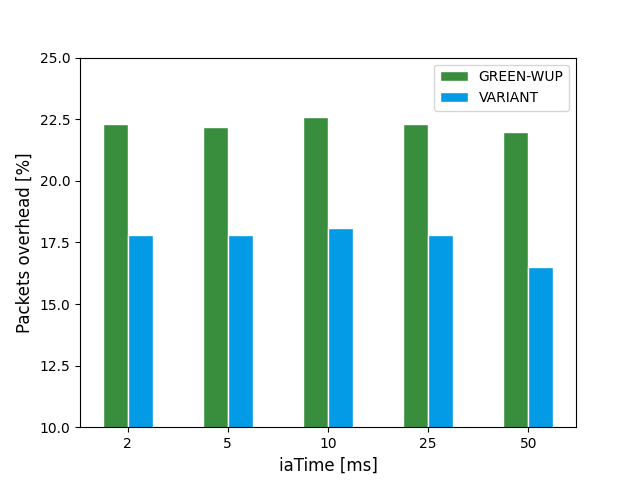
\includegraphics[width=1\linewidth]{overhead_plot.png}
        \caption*{(a)}
    \end{minipage}%
    \begin{minipage}{.5\textwidth}
        \centering
        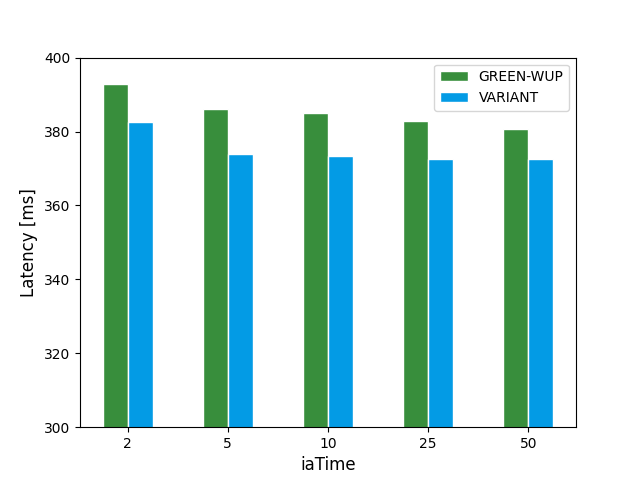
\includegraphics[width=1\linewidth]{latency_plot.png}
        \caption*{(b)}
    \end{minipage}
    \caption{Comparazione fra GREEN-WUP e la variante: (a) l'overhead di rete e (b) le latenze sperimentate.}
    \label{performance-overhead}
\end{figure}

Osservando la \textbf{Figura \ref{performance-overhead}} risulta evidente che nella variante l'overhead diminuisce in quanto diminuisce il numero totale di pacchetti di
controllo inviati per garantire il corretto trasferimento dei pacchetti dati. Il numero di quest'ultimi scende dal 22.3\% medio richiesto
dall'implementazione originale di GREEN-WUP al 17.5\% medio richiesto dalla variante.\\

In particolare, il numero dei pacchetti CTS inviati è di circa il 27\% in meno rispetto al precedente approccio e ciò segue dal fatto che un minor
numero di nodi viene coinvolto ad ogni step di selezione del nodo intermedio. In altri termini, con la variante proposta si vuole ridurre allo stretto
necessario il numero dei nodi coinvolti nella selezione del \emph{relay node} e contemporaneamente evitare sprechi energetici.\\

Conseguentemente, la latenza media richiesta per far recapitare un pacchetto (DATA) al sink node è più bassa nella variante, in quanto minore il
numero di pacchetti in circolazione, ovvero nei buffer dei nodi della rete. In particolare, la fase di ricerca dei nodi può estendersi per più tempo
in quanto nella variante l'insieme dei nodi candidati risulta essere ulteriormente partizionato, tuttavia questo è bilanciato dal fatto che i tempi
di selezione dei nodi disponibili diminuisce, favorendo quindi latenze più basse. Quest'ultima osservazione in particolare segue dal fatto che la variante
tenta di ridurre il numero di ritrasmissioni di pacchetti a causa di collisioni ed in particolare punta a ridurre il numero di pacchetti di controllo
(RTS/CTS) persi a causa del verificarsi di queste ultime.\\

\begin{figure}
    \centering
    \begin{minipage}{.5\textwidth}
        \centering
        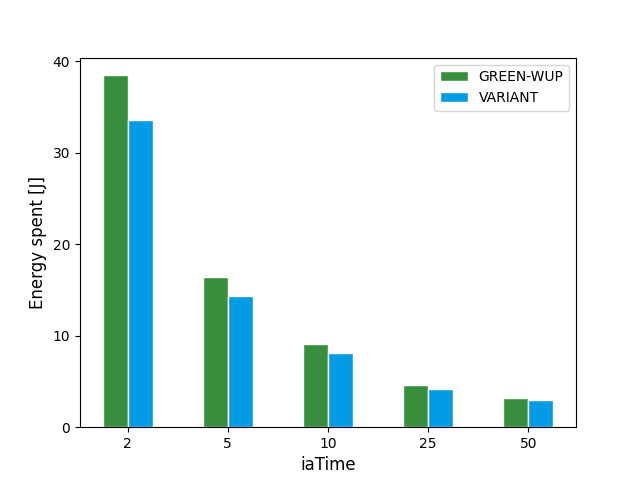
\includegraphics[width=1\linewidth]{energy_plot.png}
        \caption*{(a)}
    \end{minipage}%
    \begin{minipage}{.5\textwidth}
        \centering
        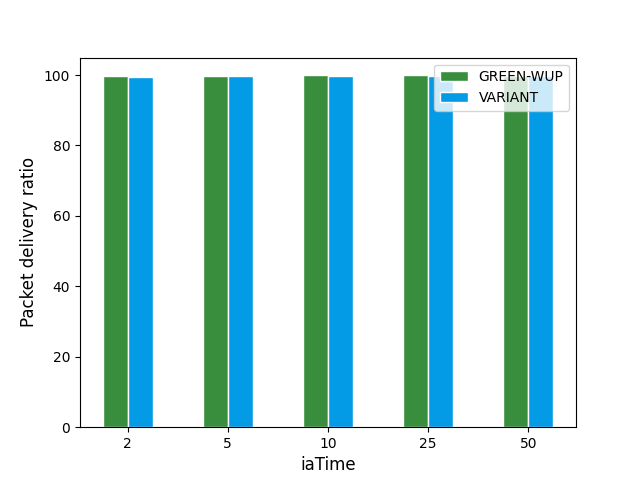
\includegraphics[width=1\linewidth]{pdr_plot.png}
        \caption*{(b)}
    \end{minipage}
    \caption{Comparazione fra GREEN-WUP e la variante: (a) l'energia spesa dalla rete e (b) il packet delivery ratio.}
    \label{performance-energy}
\end{figure}

Analizzando la \textbf{Figura \ref{performance-energy}} si può notare come l'energia richiesta dalla rete risulti essere inferiore nel caso della variante
proposta. Come diretta conseguenza di quanto sopra esposto, i consumi energetici risultano ridotti in quanto i nodi della rete che rispondono alle sequenze
di wake up con sematic addressing attivando la radio principale (RX) sono tipicamente in numero inferiore rispetto alla versione originale.\\

In termini assoluti, la massima efficienza energetica è chiaramente raggiunta in condizioni di elevato stress della rete in quanto più probabile
che un maggior numero di nodi sia svegliato in seguito alla ricezione di sequenze di wake up. In altri termini, la rete subisce un forte aumento
dei pacchetti in circolazione, e quindi di messaggi di wake up, ed in questo scenario gli effetti della modifica che permette ai nodi di
scegliere se attivare o meno la radio principale risulta essere ancor più evidente. Si noti come il miglioramento energetico sperimentato
risulti essere sempre almeno pari al 7\% e mediamente si aggira attorno al 10\%.\\

%\newpage

L'efficienza energetica della rete è favorita non solo da quest'ultima modifica ma anche dalla stessa applicazione di jitter che vengono
calcolati a partire dallo stato dei nodi e che non sono puramente randomici come nel caso dell'implementazione originale di GREEN-WUP.\\

Si noti come in \textbf{(b)} il \emph{Packet Delivery Ratio} ottenuto della variante sia mediamente dello 0.2\% inferiore rispetto a quello ottenuto
della versione originale. Questo segue dal fatto che, come discusso in \textbf{Capitolo 4.1}, esiste una probabilità che i nodi non si
sveglino a seguito della ricezione di un messaggio di wake up a loro destinato e può quindi accadere che il pacchetto dati venga scartato in seguito
al raggiungimento del numero massimo di ritrasmissioni. Nel \textbf{Capitolo 6} sono presentate alcune particolari osservazioni riguardanti
l'ottimizzazione di parametri del protocollo che puntano a migliorare alcuni aspetti delle prestazioni ottenute.\\

Infine viene fornita un'implementazione della fase di interest dissemination sia per GREEN-WUP che per la variante proposta. Si noti come i consumi
derivati dall'introduzione di questa fase siano di ordini di grandezza inferiori rispetto ai costi energetici dovuti al normale funzionamento della rete.
Inoltre, per ragioni di efficienza durante l'implementazione di questa nuova fase si è scelto di distinguere i pacchetti \emph{DATA}, utilizzati
durante la fase di scambio dati, dai pacchetti \emph{INTEREST}. Questo dettaglio implementativo garantisce che i pacchetti che realizzano la
fase di interest dissemination possano essere scambiati solamente in un primo momento della simulazione e successivamente saranno scartati.\\

Si noti come per confrontare le prestazioni ottenute dall'introduzione della fase di interest dissemination si faccia riferimento all'aspetto energetico in
quanto influenzato, anche se in piccola parte, da questa fase. Infatti durante le sperimentazioni si è osservato come gli hop count determinati
coincidono con quelli stimati dalla versione del protocollo che non esegue interest dissemination. Conseguentemente anche le latenze sperimentate
e in generale le prestazioni della rete, ad eccezione dell'energia spesa, rimangono inalterate.

\newpage

\begin{figure}
    \centering
    \begin{minipage}{.5\textwidth}
        \centering
        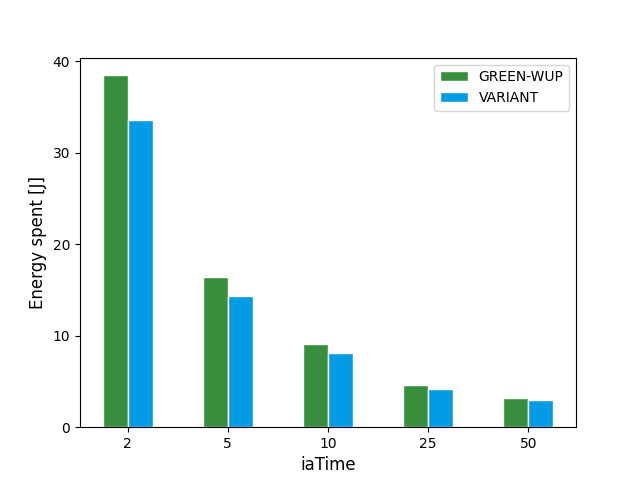
\includegraphics[width=1\linewidth]{energy_plot.png}
        \caption*{(a)}
    \end{minipage}%
    \begin{minipage}{.5\textwidth}
        \centering
        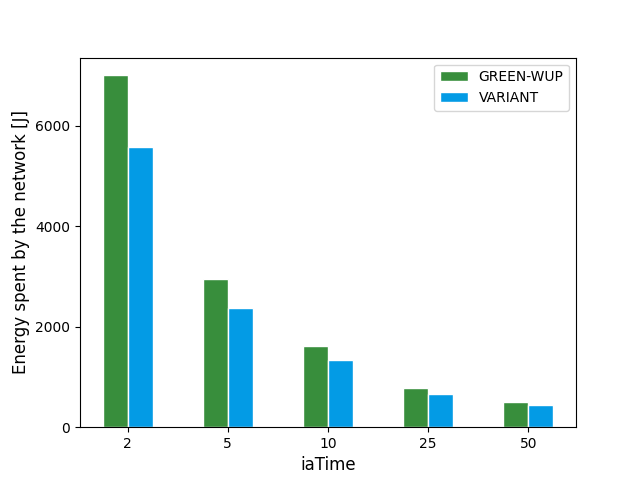
\includegraphics[width=1\linewidth]{interest_energy_plot.png}
        \caption*{(b)}
    \end{minipage}
    \caption{Comparazione dei consumi energetici di GREEN-WUP e della variante: senza (a) e con (b) la fase di interest dissemination.}
    \label{interest-plot}
\end{figure}

Osservando \textbf{Figura \ref{interest-plot} (b)}, si può notare che i consumi energetici sono appena superiori rispetto alla versione senza la fase di interest dissemination
\textbf{(a)}. In effetti, in tutte le sperimentazioni attuate l'overhead energetico registrato da ciascun nodo risulta essere costantemente al di sotto del
joule per ciascun valore assunto dal parametro $\emph{iaTime}=\{2,5,10,25,50\}$.\\

In generale i consumi energetici aggiuntivi richiesti da questa ulteriore fase possono essere considerati costanti in quanto essa viene eseguita soltanto una
volta prima dell'inizio della fase di scambio dati. Chiaramente i consumi energetici richiesti da questa fase aumentano al crescere del
numero di ripetizioni dell'invio del command packet dal momento che ciascun command packet induce alla ripetizione di una
nuova fase di scambio di pacchetti.\\

\chapter{Ottimizzazione dei parametri}

In questo capitolo verranno studiati i principali parametri che hanno influenzato i risultati e le prestazioni delle simulazioni eseguite nell'ambito di
questo lavoro. In particolare i risultati di seguito esposti fanno riferimento all'implementazione originale di GREEN-WUP descritta nel \textbf{Capitolo 3}.\\

Le prestazioni degli algoritmi impiegati nelle Wireless Sensor Network tengono conto di una moltitudine di fattori che possono influenzarne in
maniera importante i risultati raggiunti. Nel seguito verranno presentati alcuni tra questi parametri che in maggior misura contribuiscono alle
prestazioni del protocollo in questione.

\section{Scelta dei valori di jitter}

In primo luogo troviamo il parametro che misura il contingente di tempo necessario alla trasmissione di un pacchetto CTS da parte dei nodi intermedi. Da
questo punto in poi ci riferiremo al suddetto parametro come \emph{ctsMaxJitter}. Il \emph{ctsMaxJitter} viene introdotto originariamente per
aggiungere un jitter randomico alla trasmissione dei pacchetti \emph{Clear To Send}, quindi per evitare che avvengano delle collisioni dovute a multiple
trasmissioni di pacchetti nello stesso momento da parte dei nodi della rete. Possiamo vedere tale parametro come una finestra temporale all'interno
della quale ciascun nodo sceglie randomicamente un tempo $t \in [0, ctsMaxJitter]$ a cui inviare il pacchetto richiesto. Tale finestra, se sufficientemente
ampia, permette ai nodi di selezionare momenti di trasmissione diversi per inviare i pacchetti CTS.\\

Nei protocolli di rete la scelta di un buon valore di jitter è di fondamentale importanza per garantire che le prestazioni siano ottimali. Si osservi
come elevati valori di jitter comportino l'aumento della latenza media richiesta per far recapitare i pacchetti al sink node. Dualmente
scegliere un valore di jitter troppo piccolo può comportare il degrado delle prestazioni della rete a causa delle collisioni che questo comporta.
Quest'ultima condizione in particolare comporta un numero ulteriore di ritrasmissioni per far recapitare i pacchetti non ricevuti al nodo destinatario.\\

Nel seguito verranno analizzati i risultati ottenuti al variare dei valori assunti dal parametro $\emph{ctsMaxJitter}=\{25,50,100,150\}$. Si noti come
questi valori espressi in millisecondi rappresentino il massimo valore di jitter che i nodi possono attendere prima di inviare il pacchetto \emph{Clear To Send}.

\begin{figure}[h]
    \centering
    \begin{minipage}{.5\textwidth}
        \centering
        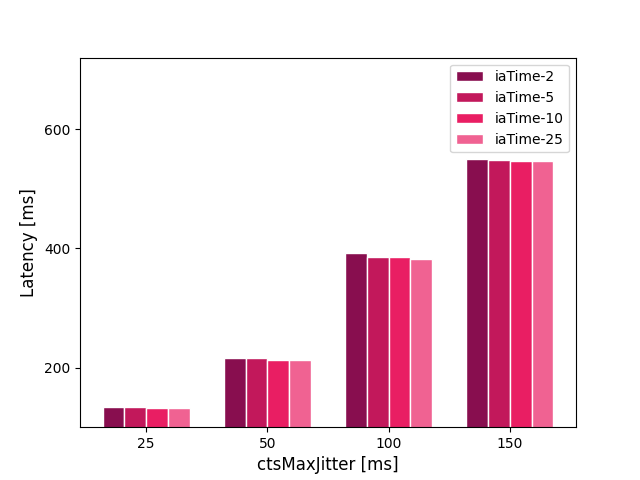
\includegraphics[width=1\linewidth]{latency_jitter_comparison_plot.png}
        \caption*{(a)}
    \end{minipage}%
    \begin{minipage}{.5\textwidth}
        \centering
        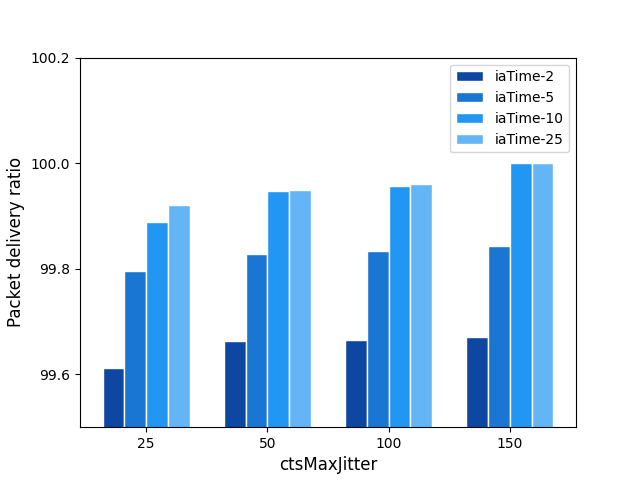
\includegraphics[width=1\linewidth]{pdr_jitter_comparison_plot.png}
        \caption*{(b)}
    \end{minipage}
    \caption{Confronto delle prestazioni del protocollo al variare del parametro \emph{ctsMaxJitter}.}
    \label{comparison-cts-latency}
\end{figure}

Come sopra anticipato, è possibile osservare in \textbf{Figura \ref{comparison-cts-latency}} che l'introduzione di un jitter impatta direttamente sulle
latenze sperimentate dalla rete. In particolare, al crescere del valore di jitter impiegato crescono i tempi di attesa per far recapitare il pacchetto al sink node.
Si noti inoltre come le latenze diminuiscono al diminuire del traffico presente in rete, ovvero al crescere del valore assunto da inter-arrival time (\emph{iaTime}).\\

Analizzando \textbf{(b)} si può inoltre notare come il \emph{Packet Delivery Ratio} risenta dei valori di jitter selezionati, raggiungendo valori ottimali per
alti valori di \emph{ctsMaxJitter}. Ciò è una diretta conseguenza del fatto che i nodi hanno una probabilità maggiore che i pacchetti da loro inviati siano
recapitati dal nodo destinatario e di ricevere quindi degli \emph{acknowledgement packet}.

\begin{figure}
    \begin{center}
        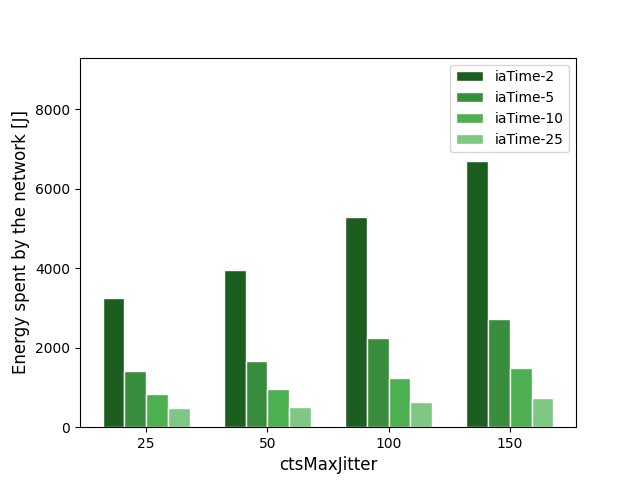
\includegraphics[scale=0.5]{energy_jitter_comparison_plot.png}
        \caption{Confronto dei consumi energetici del protocollo al variare del parametro \emph{ctsMaxJitter}.}
        \label{comparison-cts-energy}
    \end{center}
\end{figure}

Continuiamo l'analisi degli effetti del parametro \emph{ctsMaxJitter} mostrandone l'influenza rispetto ad un'altra metrica: i consumi energetici della rete. In
particolare, i consumi di energia della rete dipendono sia dal traffico in essa presente che dal valore di jitter selezionato per i nodi della rete. Osservando
\textbf{Figura \ref{comparison-cts-energy}} si può notare come questi aumentino al crescere della quantità di pacchetti in circolazione, raggiungendo il
massimo in corrispondenza di $\emph{ctsMaxJitter}=150ms$.\\

Ricordiamo che un aspetto fondamentale analizzando in consumi energetici delle reti consiste nell'attesa che precede l'invio dei pacchetti. In particolare essa
consiste in un'operazione di \emph{carrier sensing} del canale di comunicazione per verificare che nessun nodo abbia precedentemente iniziato a trasmettere dati.
Dunque, i nodi intermedi rispondono inviando un pacchetto CTS con un jitter randomico che è proporzionale al valore di \emph{ctsMaxJitter} ed è da esso superiormente
limitato. La durata del carrier sensing dipende quindi dalla durata del jitter che i nodi intermedi hanno selezionato, in quanto essi prima di poter inviare un nuovo
pacchetto devono necessariamente attendere il tempo richiesto affinché i nodi intermedi inizino a trasmettere il pacchetto CTS. Ne consegue che al crescere del
parametro \emph{ctsMaxJitter} vengono prolungate le attività di ascolto (RX) dei nodi prima che questi possano iniziare a trasmettere e quindi i consumi energetici
della rete subiscono un aumento.\\

\newpage
Risulta quindi evidente che la scelta di questo parametro non è un'operazione banale e in ambienti reali può portare ad ottenere risultati fortemente diversi tra di loro.
In generale questo è uno degli esempi di trade-off che vengono costantemente affrontati in ambito di reti ed è di vitale importanza in questi casi valutare
la metrica di riferimento che si intende ottimizzare.

\section{Trasmissioni per classe energetica}

In questa sezione discuteremo gli effetti di trasmettere più volte un pacchetto dati, riferendoci alla metrica impiegata attraverso il parametro
\emph{energyClassRetries}. Esso controlla il grado di ritrasmissione di un pacchetto da parte dei nodi della rete.\\

Il protocollo GREEN-WUP si basa sull'assunzione che la rete sottostante sia di tipologia \emph{multi-hop} e che i percorsi di rete da seguire non siano noti a priori.
In particolare, se un nodo genera un pacchetto da far recapitare al sink node allora la comunicazione coinvolgerà più nodi intermedi che si faranno
carico di ritrasmettere il pacchetto verso il sink node. La scelta dei nodi intermedi è condizionata ogni volta dalla scelta del nodo che gode
di una buona disponibilità energetica e, una volta che questo è stato individuato, si procede poi ritrasmettendolo a quello specifico nodo. Se tuttavia
il nodo non è stato individuato si procede considerando i nodi con classe energetica inferiore sino a che questo non è stato trovato. \\

Analizzando quanto appena descritto è evidente che la scelta \emph{greedy} di un nodo intermedio secondo questi termini non sia ottimale in termini di prestazioni
della rete. Infatti è possibile che un nodo, a seguito di un congestionamento del canale di comunicazione oppure a causa della sua temporanea indisponibilità
non sia momentaneamente in grado di ricevere un nuovo pacchetto. Vale quindi la pena analizzare il comportamento della rete introducendo un numero massimo di
tentativi che ciascun nodo dispone per trasmettere il pacchetto ad una specifica classe energetica. Si noti come l'introduzione di questo parametro non
comporti necessariamente variazioni nella latenza media sperimentata dalla rete, in quanto essa considera i pacchetti ricevuti dal sink node ed è definita
dal tempo medio che questo ha richiesto per essere ricevuto. In altri termini, un pacchetto scartato a seguito di aver superato il numero massimo
di ritrasmissioni non viene considerato nel calcolo della latenza media sperimentata dalla rete dal momento che il sink node non lo ha mai ricevuto.

\begin{figure}[h]
    \centering
    \begin{minipage}{.5\textwidth}
        \centering
        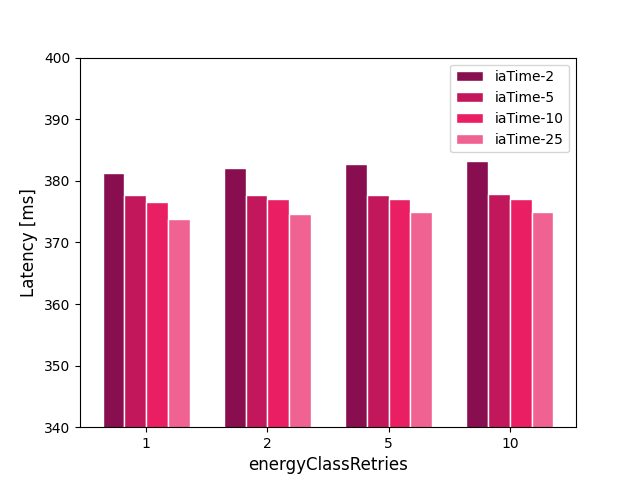
\includegraphics[width=1\linewidth]{latency_retries__comparison_plot.png}
        \caption*{(a)}
    \end{minipage}%
    \begin{minipage}{.5\textwidth}
        \centering
        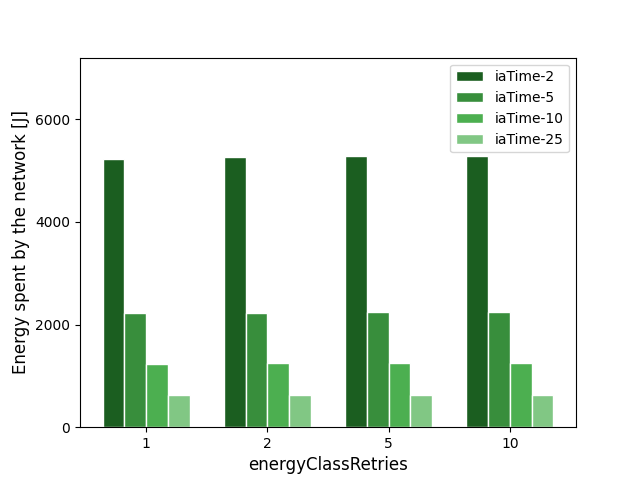
\includegraphics[width=1\linewidth]{energy_retries__comparison_plot.png}
        \caption*{(b)}
    \end{minipage}
    \begin{minipage}{.5\textwidth}
        \centering
        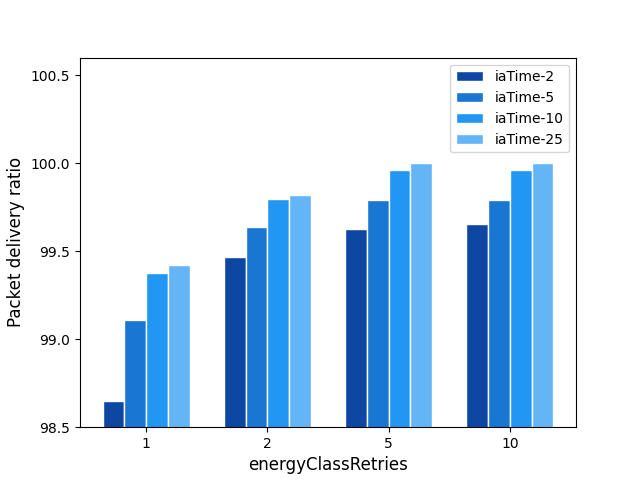
\includegraphics[width=1\linewidth]{pdr_retries__comparison_plot.png}
        \caption*{(c)}
    \end{minipage}
    \caption{Confronto delle prestazioni del protocollo al variare del parametro \emph{energyClassRetries}.}
    \label{comparison-retries}
\end{figure}

È interessante notare in \textbf{Figura \ref{comparison-retries}} che per quanto sopra osservato le latenze medie \textbf{(a)} non sono influenzate in
maniera significativa dal parametro \emph{energyClassRetries}. Infatti nello scenario considerato abbiamo osservato che esse sono influenzate essenzialmente dai
tempi di trasmissione dei pacchetti e dai tempi di attesa previsti dal protocollo.\\

In particolare, ciascun pacchetto dispone di un numero massimo di trasmissioni $n$ ed un numero massimo di ritrasmissioni per classe energetica
$\emph{energyClassRetries} \leq n$ che, seppur fanno riferimento ad comportamenti simili, modellano aspetti diversi. Il primo fornisce un limite al
numero di volte che i nodi provano ad inviare gli stessi pacchetti e serve quindi ad evitare che questi rimangano bloccati nel processamento dello stesso pacchetto
per un tempo indefinito. Il secondo invece permette ai nodi riceventi di disporre di più tentativi per la ricezione dei pacchetti, favorendo in maniera indiretta
i nodi di classe energetica superiore in quanto considerati in ordine decrescente di classe energetica. Risulta quindi evidente che essi svolgono
un ruolo vitale nel regolamentare il comportamento dei protocolli di rete, in quanto un'errata scelta di questi due valori può portare ad un crollo
delle prestazioni della rete. Ad esempio, alti valori di $n$ possono portare ad aumenti considerevoli nei consumi energetici fino anche alla morte di
nodi della rete a seguito del loro scaricamento.\\

Conseguentemente in \textbf{(b)} si può notare come i consumi energetici della rete crescano, seppur in maniera lieve, al crescere di \emph{energyClassRetries}.
Questo accade poiché i nodi della rete sono attivi per più tempo dal momento che dispongono più tentativi di trasmettere i pacchetti.\\

Si noti infine come in \textbf{(c)} le prestazioni della rete risentano maggiormente del valore di \emph{energyClassRetries} scelto. Il \emph{packet delivery ratio}
tocca il valore minimo di 98.8\% in prossimità di $\emph{energyClassRetries}=1$ e di elevate condizioni di stress della rete. Chiaramente la metrica considerata
è influenzata dallo stato di traffico della rete come pure dal numero di tentativi per classe energetica poiché regola la profondità a cui ciascuna classe
energetica viene analizzata. Infatti, per quanto osservato alcuni nodi di una classe energetica potrebbero non essere considerati in una prima fase di analisi
ma essere successivamente disponibili. Da questo segue che una volta esaminate tutte le classi energetiche il pacchetto considerato viene scartato, portando
ad una diminuzione dei valori del \emph{packet delivery ratio}.\\

In generale un cattiva scelta del parametro \emph{energyClassRetries} può condurre al degrado delle prestazioni della rete. Tuttavia si noti in \textbf{(c)}
come nelle simulazioni eseguite l'aumento del valore di PDR subisca un forte rallentamento una volta raggiunto il valore $\emph{energyClassRetries}=5$. Ne
consegue quindi che le prestazioni crescono in maniera proporzionale al valore di \emph{energyClassRetries} scelto fino ad una certa soglia e
successivamente smettono di migliorare.

\chapter{Conclusioni}

In questo lavoro abbiamo presentato lo scenario delle Wireless Sensor Network ed esplorato il loro aspetto \emph{green} che coinvolge le tecnologie di
wake up radio, semantic addressing e energy harvesting. Abbiamo inoltre affrontato sia l'aspetto teorico delle problematiche comuni ai protocolli per sistemi IoT
sia quello pratico in riferimento alla loro presenza nel protocollo GREEN-WUP. Successivamente abbiamo proposto una nuova variante di GREEN-WUP
che affronta i problemi del protocollo originale ed infine abbiamo valutato i risultati raggiunti in un'ottica di ottimizzazione dei parametri fondamentali
che contribuiscono a regolarne i comportamento al fine di migliorare le prestazioni ottenute.\\

Durante questo lavoro di tirocinio abbiamo studiato i protocolli per dispositivi IoT, studiandone l'aspetto teorico e analizzandole le prestazioni. In futuro
sarebbe sicuramente interessante introdurre nuove variazioni al protocollo GREEN-WUP che modellano l'esigenza di ottimizzare ulteriormente i consumi energetici
e le latenze sperimentate. Inoltre vale la pena analizzare le prestazioni che il protocollo raggiunge quando sottoposto a nuove condizioni di traffico o dello
stato della rete (es. nodi altamente congestionati, link di trasmissione meno performanti). Nel corso della tesi sono state effettuate prime valutazioni prestazionali
che hanno portato ad un primo insieme di ottimizzazioni e varianti, attività che potrebbe essere estesa per sviluppare nuovi protocolli e analizzare completamente
lo spazio dei parametri per ottimizzarli. Infine il SENSES Lab ha realizzato un testbed per reti IoT dotate di wake up radio. Una volta consolidate le varianti e
le ottimizzazioni dei protocolli sarebbe interessante valutarne sperimentalmente le prestazioni mediante un testbed in ambiente reale.


\backmatter
\cleardoublepage
\phantomsection % Give this command only if hyperref is loaded
\addcontentsline{toc}{chapter}{\bibname}

\begin{thebibliography}{9}

    \bibitem{novel-wake-up-receiver-paper}
    C. Petrioli, D. Spenza, P. Tommasino, A. Trifiletti.
    \say{A Novel Wake-Up Receiver with Addressing Capability for Wireless Sensor Nodes}.
    In: \textit{2014 IEEE International Conference on Distributed Computing in Sensor Systems. Marina Del Rey, CA, USA, May 26-28 2014.}

    \bibitem{beyond-duty-cycling-paper}
    D. Spenza, M. Magno, S. Basagni, L. Benini, M. Paoli, C. Petrioli.
    \say{Beyond duty cycling: Wake-up radio with selective awakenings for long-lived wireless sensing systems}.
    In: \textit{2015 IEEE Conference on Computer Communications (INFOCOM). Kowloon, Hong Kong, April 26-May 1 2015.}

    \bibitem{ctp-wur-paper}
    S. Basagni, C. Petrioli, D. Spenza.
    \say{CTP-WUR: The collection tree protocol in wake-up radio WSNs for critical applications}.
    In: \textit{2016 International Conference on Computing, Networking and Communications (ICNC). Kauai, HI, USA, February 15-18 2016.}

    \bibitem{energy-harvesting-paper}
    S. Basagni, G. Koutsandria, C. Petrioli.
    \say{A Comparative Performance Evaluation of Wake-Up Radio-Based Data Forwarding for Green Wireless Networks}.
    In: \textit{2018 27th International Conference on Computer Communication and Networks (ICCCN). Hangzhou, China, July 30-August 2 2018}.

    \bibitem{wake-up-radios-paper}
    S. Basagni, V. Di Valerio, G. Koutsandria, C. Petrioli.
    \say{Wake-up Radio-enabled Routing for Green Wireless Sensor Networks}.
    In: \textit{2017 IEEE 86th Vehicular Technology Conference (VTC-Fall). Toronto, ON, Canada, September 24-27 2017}.

    \bibitem{wsn-energy-harvesting-paper}
    S. Basagni, M. Y. Naderi, C. Petrioli, D. Spenza.
    \say{Wireless Sensor Networks with energy harvesting}.
    In: \textit{Mobile Ad Hoc Networking: The Cutting Edge Directions. Hoboken, NJ, 2013}.

    \newpage        % do not cut references

    \bibitem{hop-count-figure}
    J. H. Feng, Y. Sun, R. Sun, W. Chen, S. Ma, J. Gao.
    \say{A Distributed Energy Optimized Routing Using Virtual Potential Field in Wireless Sensor Networks}.
    In: \textit{International Journal of Distributed Sensor Networks. July 2014.}

    \bibitem{greencastalia-paper}
    D. Benedetti, C. Petrioli, D. Spenza.
    \say{GreenCastalia: An Energy-Harvesting-Enabled Framework for the Castalia Simulator}.
    In: \textit{Proceeding of the ACM 1st International Workshop on Energy Neutral Sensing Systems, ACM ENSSys 2013. Rome, Italy, November 11-14 2013.}

    \bibitem{wharp-paper}
    S. Basagni, V. Di Valerio, G. Koutsandria, C. Petrioli, D. Spenza.
    \say{WHARP: A Wake-Up Radio and Harvesting-Based Forwarding Strategy for Green Wireless Networks}.
    In: \textit{2017 IEEE 14th International Conference on Mobile Ad Hoc and Sensor Systems (MASS). Orlando, FL, USA, October 22-25 2017.}

    \bibitem{magonode-pp-paper}
    M. Paoli, D. Spenza, C. Petrioli, M. Magno, L. Benini.
    \say{MagoNode++: A Wake-Up-Radio-Enabled Wireless Sensor Mote for Energy-Neutral Applications}.
    In: \textit{2016 15th ACM/IEEE International Conference on Information Processing in Sensor Networks (IPSN). Vienna, Austria, April 11-14 2016.}

\end{thebibliography}

\end{document}